\begin{tikzpicture}[
    node distance=1.3cm and 1.2cm,
    % --- STYLES ---
    input_item_box/.style={rectangle, rounded corners, draw=bordergray, minimum height=0.5cm, minimum width=4.8cm, align=center, thick},
    process_box/.style={rectangle, rounded corners, draw=borderblue, fill=processblue, minimum height=2.5cm, minimum width=4cm, align=center, text width=3.8cm, thick},
    transformer_box/.style={rectangle, rounded corners, draw=borderpurple, fill=modelpurple, minimum height=2.5cm, minimum width=4cm, align=center, text width=3.8cm, thick},
    transformer_box_frozen/.style={rectangle, rounded corners, draw=borderpurple!50, fill=modelpurple!40, minimum height=2.5cm, minimum width=4cm, align=center, text width=3.8cm, thick},
    aux_transformer_box/.style={rectangle, rounded corners, draw=borderteal, fill=taskteal, minimum height=2.0cm, minimum width=3.5cm, align=center, text width=3.3cm, thick},
    output_box_gen/.style={rectangle, rounded corners, draw=borderblue, fill=processblue, minimum height=0.5cm, minimum width=3.4cm, align=center, thick},
    output_box_aux/.style={rectangle, rounded corners, draw=borderoutputgreen, fill=outputgreen, minimum height=0.5cm, minimum width=3.4cm, align=center, thick},
    group_box/.style={rectangle, rounded corners, draw=none, inner sep=0.0cm},
    stage_label/.style={font=\Large\bfseries, color=black!70},
    arrow/.style={->, thick, >=stealth, rounded corners=5pt},
    arrow_dashed/.style={->, thick, >=latex, dashed, black!70, rounded corners=15pt},
    checklist_box/.style={rectangle, rounded corners, draw=bordergray, fill=inputgray, align=left, text width=3.8cm, thick, font=\small, inner sep=3pt}
]

    % --- STAGE 1: PRETRAINING ---
    \begin{scope}[local bounding box=stage1]
        \node (input_pos_ref) at (0, 2.5) {}; % Invisible node for positioning
        \node[input_item_box, below=0.0cm of input_pos_ref] (in1) {Atom types (B, N, 1) $\sim \text{Cat}(t)$};
        \node[input_item_box, below=0.1cm of in1] (in2) {3D coord. (B, N, 3) + $\epsilon(t)$};
        \node[input_item_box, below=0.1cm of in2] (in3) {Frac. coord. (B, N, 3) + $\epsilon(t)$};
        \node[input_item_box, below=0.1cm of in3] (in4) {Cell lengths (B, 1, 3) + $\epsilon(t)$};
        \node[input_item_box, below=0.1cm of in4] (in5) {Cell angles (B, 1, 3) + $\epsilon(t)$};
        \node[input_item_box, below=0.1cm of in5] (in6) {Class label (B, 1, 1)};
        \node[input_item_box, below=0.1cm of in6] (in7) {Time $t$ (B, 1, 1)};

        % Invisible node to group inputs for arrow connection
        \node[fit=(in1)(in7), inner sep=0pt] (inputs) {};

        % Rotated Title
        \node[rotate=90, left=0.6cm of inputs, anchor=center] (input_title) {\textbf{\textcolor{black!70}{Noisy input representation}}};

        % --- CENTRAL PATH ---
        \node[process_box, right=of inputs] (embedding) {\textbf{Input Embedding} \\ \& \textbf{Positional Encoding} \\ \vspace{0.7cm}};

        \node[transformer_box, right=of embedding] (transformer_stack) {\textbf{Transformer Trunk} \\ \vspace{0.2cm} $L$ layers, \\ multi-head self-attention};

        % --- VISUALIZATION OF MULTI-HEAD ATTENTION ---
        \begin{scope}[on background layer]
            \node[transformer_box, anchor=center] at ($(transformer_stack.center)+(0.12,0.12)$) {};
            \node[transformer_box, anchor=center] at ($(transformer_stack.center)+(0.06,0.06)$) {};
        \end{scope}

        \draw[arrow] (inputs) -- (embedding);
        \draw[arrow] (embedding) -- (transformer_stack);

        % --- GENERATIVE PATH (RIGHT SIDE) ---
        \node[output_box_gen, right=1.8cm of transformer_stack] (out_frac_coords) {Frac. coord. (B, N, 3)};
        \node[output_box_gen, above=0.2cm of out_frac_coords] (out_3d_coords) {3D coord. (B, N, 3)};
        \node[output_box_gen, above=0.2cm of out_3d_coords] (out_atom_types) {Atom types (B, N, 1)};
        \node[output_box_gen, below=0.2cm of out_frac_coords] (out_cell_lengths) {Cell lengths (B, 1, 3)};
        \node[output_box_gen, below=0.2cm of out_cell_lengths] (out_cell_angles) {Cell angles (B, 1, 3)};

        \coordinate (gen_bus) at ($(transformer_stack.east)!0.5!(out_frac_coords.west)$);
        \draw[arrow,-] (transformer_stack.east) -- (gen_bus);
        \draw[-] (gen_bus |- out_atom_types.west) -- (gen_bus |- out_cell_angles.west);

        \draw[arrow] (gen_bus |- out_atom_types.west) -- (out_atom_types.west);
        \draw[arrow] (gen_bus |- out_3d_coords.west) -- (out_3d_coords.west);
        \draw[arrow] (gen_bus |- out_frac_coords.west) -- (out_frac_coords.west);
        \draw[arrow] (gen_bus |- out_cell_lengths.west) -- (out_cell_lengths.west);
        \draw[arrow] (gen_bus |- out_cell_angles.west) -- (out_cell_angles.west);

        \node[group_box, fit=(out_atom_types)(out_cell_angles), label={[yshift=0.25cm]above:\textbf{Generative Heads}}] (generative_group) {};

        % --- ADDED: RESIDUAL CONNECTION FOR STAGE 1 ---
        \coordinate (res1_start) at ($(embedding.east)!0.67!(transformer_stack.west)$);
        \coordinate (res1_end) at ($(transformer_stack.east)!0.5!(gen_bus)$);
        \draw[arrow] (res1_start) |- ($(transformer_stack.north) + (0, 0.5cm)$) node[above, font=\small, color=black!70] {\textbf{Residual Cross-Attention}} -| (res1_end);

        % --- EXAMPLE OUTPUTS ---
        \node (example_outputs_gen) [right=1.2cm of generative_group, align=center, font=\normalsize, color=black!70, yshift=0.5cm] {
            \textbf{Example outputs} \\[5pt]
            \begin{minipage}[c]{2.5cm}
                \centering
                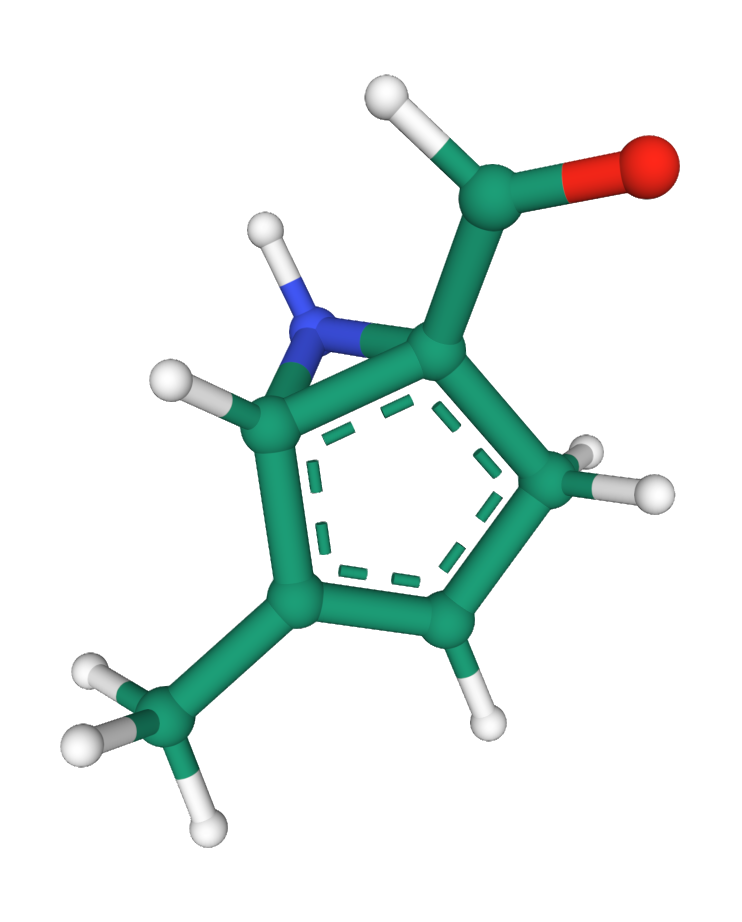
\includegraphics[width=0.6\linewidth]{figures/zatom_1_molecule.png}
                \small \textcolor{black!70}{\mbox{3D Molecule}}
            \end{minipage}
            \\[10pt]
            \begin{minipage}[c]{2.5cm}
                \centering
                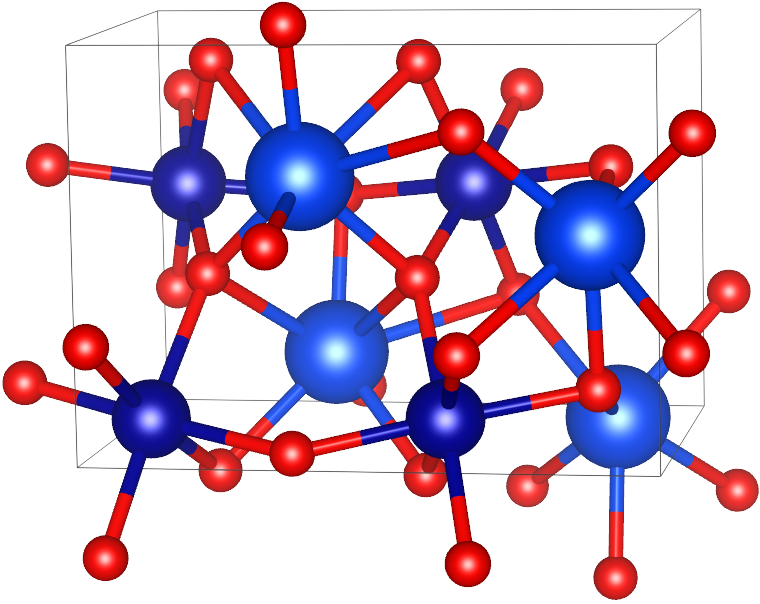
\includegraphics[width=0.8\linewidth]{figures/zatom_1_material.png}
                \small \textcolor{black!70}{\mbox{3D Material}}
            \end{minipage}
        };
    \end{scope}

    \node[group_box, fit=(stage1)(example_outputs_gen), label={[anchor=north west, xshift=0.2cm, yshift=-1.0cm]north west:\phantom{Stage 1}}] (stage1_bbox) {};
    \node[stage_label, anchor=north west, yshift=0.2cm] at (stage1_bbox.north west) {Stage 1: Pretraining (Multimodal Flow Matching)};

    % --- STAGE 2: FINETUNING ---
    \begin{scope}[local bounding box=stage2, yshift=-6.5cm]
        \node (input_ft_pos_ref) at (0, 2.5) {}; % Invisible node for positioning
        \node[input_item_box, below=0.0cm of input_ft_pos_ref] (in_ft1) {Atom types (B, N, 1)};
        \node[input_item_box, below=0.1cm of in_ft1] (in_ft2) {3D coord. (B, N, 3)};
        \node[input_item_box, below=0.1cm of in_ft2] (in_ft3) {Frac. coord. (B, N, 3)};
        \node[input_item_box, below=0.1cm of in_ft3] (in_ft4) {Cell lengths (B, 1, 3)};
        \node[input_item_box, below=0.1cm of in_ft4] (in_ft5) {Cell angles (B, 1, 3)};
        \node[input_item_box, below=0.1cm of in_ft5] (in_ft6) {Class label (B, 1, 1)};

        % Invisible node to group inputs for arrow connection
        \node[fit=(in_ft1)(in_ft6), inner sep=0pt] (inputs_ft) {};

        % Rotated Title
        \node[rotate=90, left=0.6cm of inputs_ft, anchor=center] (input_ft_title) {\textbf{\textcolor{black!70}{Input representation}}};

        % --- CENTRAL PATH ---
        \node[process_box, at=({embedding.center} |- {inputs_ft.center})] (embedding_ft) {\textbf{Input Embedding} \\ \& \textbf{Positional Encoding} \\ \vspace{0.1cm} (Frozen weights \faSnowflake)};

        \node[transformer_box_frozen, at=({transformer_stack.center} |- {inputs_ft.center})] (transformer_stack_ft) {\textbf{Transformer Trunk} \\ \vspace{0.1cm} (Frozen weights \faSnowflake)};

        % --- VISUALIZATION OF MULTI-HEAD ATTENTION ---
        \begin{scope}[on background layer]
            \node[transformer_box_frozen, anchor=center] at ($(transformer_stack_ft.center)+(0.12,0.12)$) {};
            \node[transformer_box_frozen, anchor=center] at ($(transformer_stack_ft.center)+(0.06,0.06)$) {};
        \end{scope}

        \draw[arrow] (inputs_ft) -- (embedding_ft);
        \draw[arrow] (embedding_ft) -- (transformer_stack_ft);

        % --- DOWNSTREAM PATH ---
        \node[aux_transformer_box, at=({out_frac_coords.center} |- {transformer_stack_ft.center})] (aux_backbone) {\textbf{Downstream Task Backbone} \\ \vspace{0.2cm} $M$ auxiliary layers,\\ \faFire\ per task};

        % --- VISUALIZATION OF MULTIPLE LAYERS ---
        \begin{scope}[on background layer]
            \node[aux_transformer_box, anchor=center] at ($(aux_backbone.center)+(0.12,0.12)$) {};
            \node[aux_transformer_box, anchor=center] at ($(aux_backbone.center)+(0.06,0.06)$) {};
        \end{scope}

        \coordinate (aux_takeoff) at ($(transformer_stack_ft.north east)!0.5!(transformer_stack_ft.south east)$);
        \draw[arrow] (aux_takeoff) -- (aux_backbone.west);
        \node[align=center, font=\small, color=black!70, above, xshift=0.2cm] at ($(aux_takeoff)!0.5!(aux_backbone.west)$) {Use \\ layer $K$};

        % --- ADDED: RESIDUAL CONNECTION FOR STAGE 2 ---
        \coordinate (res2_start) at ($(embedding_ft.east)!0.67!(transformer_stack_ft.west)$);
        \coordinate (res2_end) at ($(aux_takeoff)!0.25!(aux_backbone.west)$);
        \draw[arrow] (res2_start) |- ($(transformer_stack_ft.south) - (0, 0.45cm)$) node[below, font=\small, color=black!70] {\textbf{Residual Cross-Attention} \faFire} -| (res2_end);

        \node[output_box_aux, above=0.3cm of aux_backbone] (out_props) {Properties (B, 1, 19)};
        \node[output_box_aux, below=0.3cm of aux_backbone] (out_energy) {Energy (B, 1, 1)};
        \node[output_box_aux, below=0.3cm of out_energy] (out_forces) {Forces (B, N, 3)};

        \draw[arrow] (aux_backbone.north) -- (out_props.south);
        \draw[arrow, -] (aux_backbone.south) -- (out_energy.north);
        \draw[arrow] (out_energy.south) -- (out_forces.north);

        \node[group_box, fit=(out_forces)(out_props), label={[yshift=0.25cm]above:\textbf{Downstream Task Heads}}] (downstream_group) {};

        % --- EXAMPLE OUTPUTS ---
        \node (example_outputs_ft) [at=({example_outputs_gen.center} |- {downstream_group.center}), align=center, font=\normalsize, color=black!70] {
            \textbf{Example outputs} \\ \\ Energy: scalar \faCircle \vspace{0.3cm} \\ Forces: vector \faLocationArrow
        };
    \end{scope}

    \node[group_box, fit=(stage2)(example_outputs_ft), label={[anchor=north west, xshift=0.2cm, yshift=-1.0cm]north west:\phantom{Stage 2}}] (stage2_bbox) {};
    \node[stage_label, anchor=north west, yshift=0.3cm] at (stage1_bbox.north west |- stage2_bbox.north west) {Stage 2: Finetuning (Multi-Task Learning)};

    % --- CHECKLIST BOX NODE ---
    \node[checklist_box] (checklist) at ($(example_outputs_gen.south)!0.5!(example_outputs_ft.north)$) {
        \textbf{Key Model Capabilities}\\[1.5pt]
        \faCheck\ Fast to train \\
        \faCheck\ Fast to sample \\
        \faCheck\ Minimal priors \\
        \faCheck\ Molecules \& materials \\
        \faCheck\ Generation \& prediction
    };

    % --- ARROW BETWEEN STAGES ---
    \draw[arrow_dashed] (transformer_stack.south) to[out=-80,in=80] node[midway, right, align=center, font=\small] {Same \\ weights \\ --- \\ New \\ prediction \\ capabilities} (transformer_stack_ft.north);

\end{tikzpicture}